\documentclass[11pt, a4paper]{article}
\usepackage[utf8]{inputenc}
\usepackage{graphicx}
\usepackage{amsmath}
\usepackage{booktabs}
\usepackage{hyperref}
\usepackage{float}
\usepackage{subcaption}
\usepackage{geometry}
\usepackage{longtable}
\usepackage{array}

\geometry{margin=1in}

\title{\textbf{Machine Learning for Credit Score Classification:}\\A Comparative Analysis of Ensemble Methods}
\author{Davide De Blasio\\Student ID: 2082600}
\date{November 2025}

\begin{document}

\maketitle

\section{Introduction}

Credit scoring is fundamental to modern finance, enabling institutions to assess risk, determine loan eligibility, and set interest rates. Traditional methods such as FICO scores rely on limited variables and rigid rules that may not capture the full complexity of financial behavior. Machine learning offers a data-driven alternative that identifies subtle patterns and non-linear relationships across multiple behavioral and financial features.

\subsection{Motivation and Objectives}

This project develops and evaluates a comprehensive machine learning pipeline to predict customer credit scores (\textbf{Poor}, \textbf{Standard}, \textbf{Good}) using a \href{https://www.kaggle.com/datasets/parisrohan/credit-score-classification}{Kaggle Credit Score Classification Dataset} containing 100,000 records with 28 features. We compare six algorithms: Gaussian Naive Bayes, Multinomial Naive Bayes, Softmax Regression, Decision Tree, and two Random Forest variants (20 and 15 features). All models are optimized using 5-fold cross-validation with weighted F1-score as the primary metric.

The analysis focuses on four key dimensions: (1) predictive accuracy across multiple metrics, (2) model interpretability through feature importance analysis, (3) computational efficiency for practical deployment, and (4) generalization capability to unseen data. This comprehensive evaluation provides actionable insights for financial institutions seeking to implement machine learning-based credit scoring systems.

\section{Dataset Description}

The dataset used in this project consists of 100,000 customer records and originally contained 28 features including the target variable. The data represents diverse credit profiles from a publicly available Kaggle competition focused on credit score classification.

\subsection{Features and Target Variable}
The target variable, \texttt{Credit\_Score}, is categorical with three balanced classes: \textbf{Poor}, \textbf{Standard}, and \textbf{Good}, representing the customer's creditworthiness level. For modeling purposes, these classes were numerically encoded as 0, 1, and 2, respectively.

The features can be categorized as follows:
\begin{itemize}
    \item \textbf{Demographic:} Age, Occupation.
    \item \textbf{Financial:} Annual\_Income, Monthly\_Inhand\_Salary, Monthly\_Balance, Amount\_invested\_monthly, Total\_EMI\_per\_month, Outstanding\_Debt.
    \item \textbf{Credit Behavior:} Num\_Bank\_Accounts, Num\_Credit\_Card, Interest\_Rate, Credit\_Utilization\_Ratio, Credit\_History\_Age, Credit\_Mix, Changed\_Credit\_Limit.
    \item \textbf{Loan Information:} Num\_of\_Loan, Type\_of\_Loan, Delay\_from\_due\_date, Num\_of\_Delayed\_Payment.
    \item \textbf{Payment Patterns:} Payment\_of\_Min\_Amount, Payment\_Behaviour, Num\_Credit\_Inquiries.
\end{itemize}

\begin{figure}[H]
    \centering
    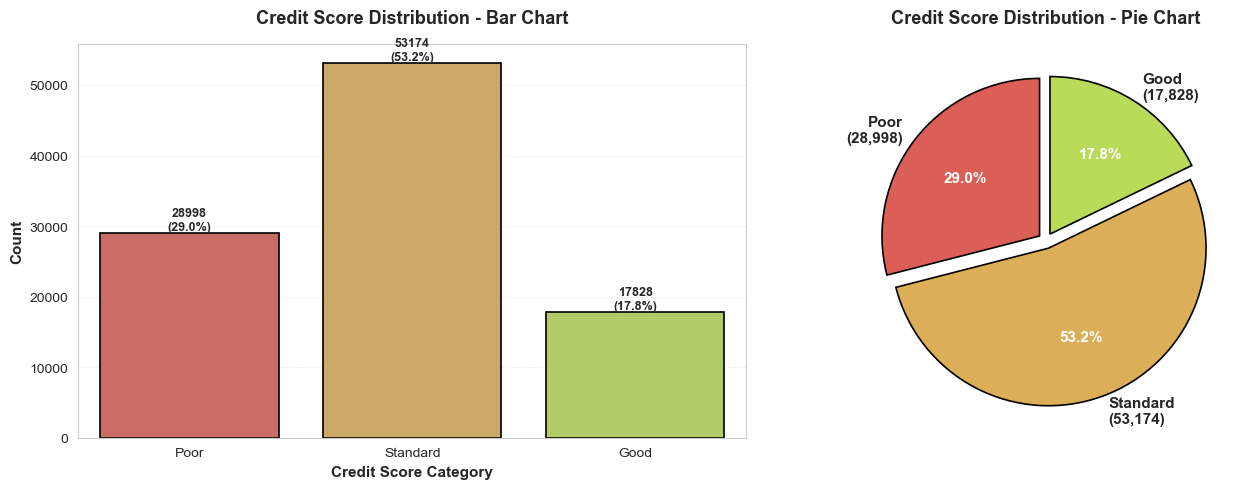
\includegraphics[width=0.8\textwidth]{size.png}
    \caption{Distribution of Target Variable (Credit Score). The dataset shows a balanced distribution across three classes: Poor, Standard, and Good, facilitating unbiased model training.}
    \label{fig:target_dist}
\end{figure}

\subsection{Preprocessing Pipeline}

A rigorous seven-stage preprocessing pipeline was applied:

\textbf{1. Data Cleaning:} Dropped irrelevant columns (ID, Name, SSN), converted string-stored numerical features to float64, replaced negative values and placeholders with NaN.

\textbf{2. Missing Value Imputation:} Customer-specific mode/median imputation with global fallback; rows with missing Type\_of\_Loan deleted.

\textbf{3. Feature Engineering:} Expanded Type\_of\_Loan into 8 binary columns, converted Credit\_History\_Age to total months, re-encoded Customer\_ID to integers.

\textbf{4. Statistical Feature Selection:} Chi-Square tests removed Month and Occupation. ANOVA F-tests eliminated three low-variance features (Monthly\_Balance, Age, Total\_EMI\_per\_month).

\textbf{5. Outlier Treatment:} IQR-based capping (from $Q_1 - 1.5 \times IQR$ to $Q_3 + 1.5 \times IQR$) preserved sample size while mitigating extreme values.

\textbf{6. Feature Encoding:} Target encoded as integers (Poor=0, Standard=1, Good=2), Credit\_Mix ordinally encoded, Payment\_Behaviour one-hot encoded with \texttt{drop\_first=True}.

\textbf{7. Final Selection and Scaling:} SelectKBest with mutual information selected top 20 features from approximately 35 features. We applied an 80-20 stratified split, using RobustScaler for most models and MinMaxScaler for Multinomial NB.

\subsection{Data Quality Impact}

The preprocessing pipeline significantly improved data quality and feature distributions. Figure \ref{fig:dist_comparison} shows the distribution comparison before and after preprocessing for key features.

\begin{figure}[H]
    \centering
    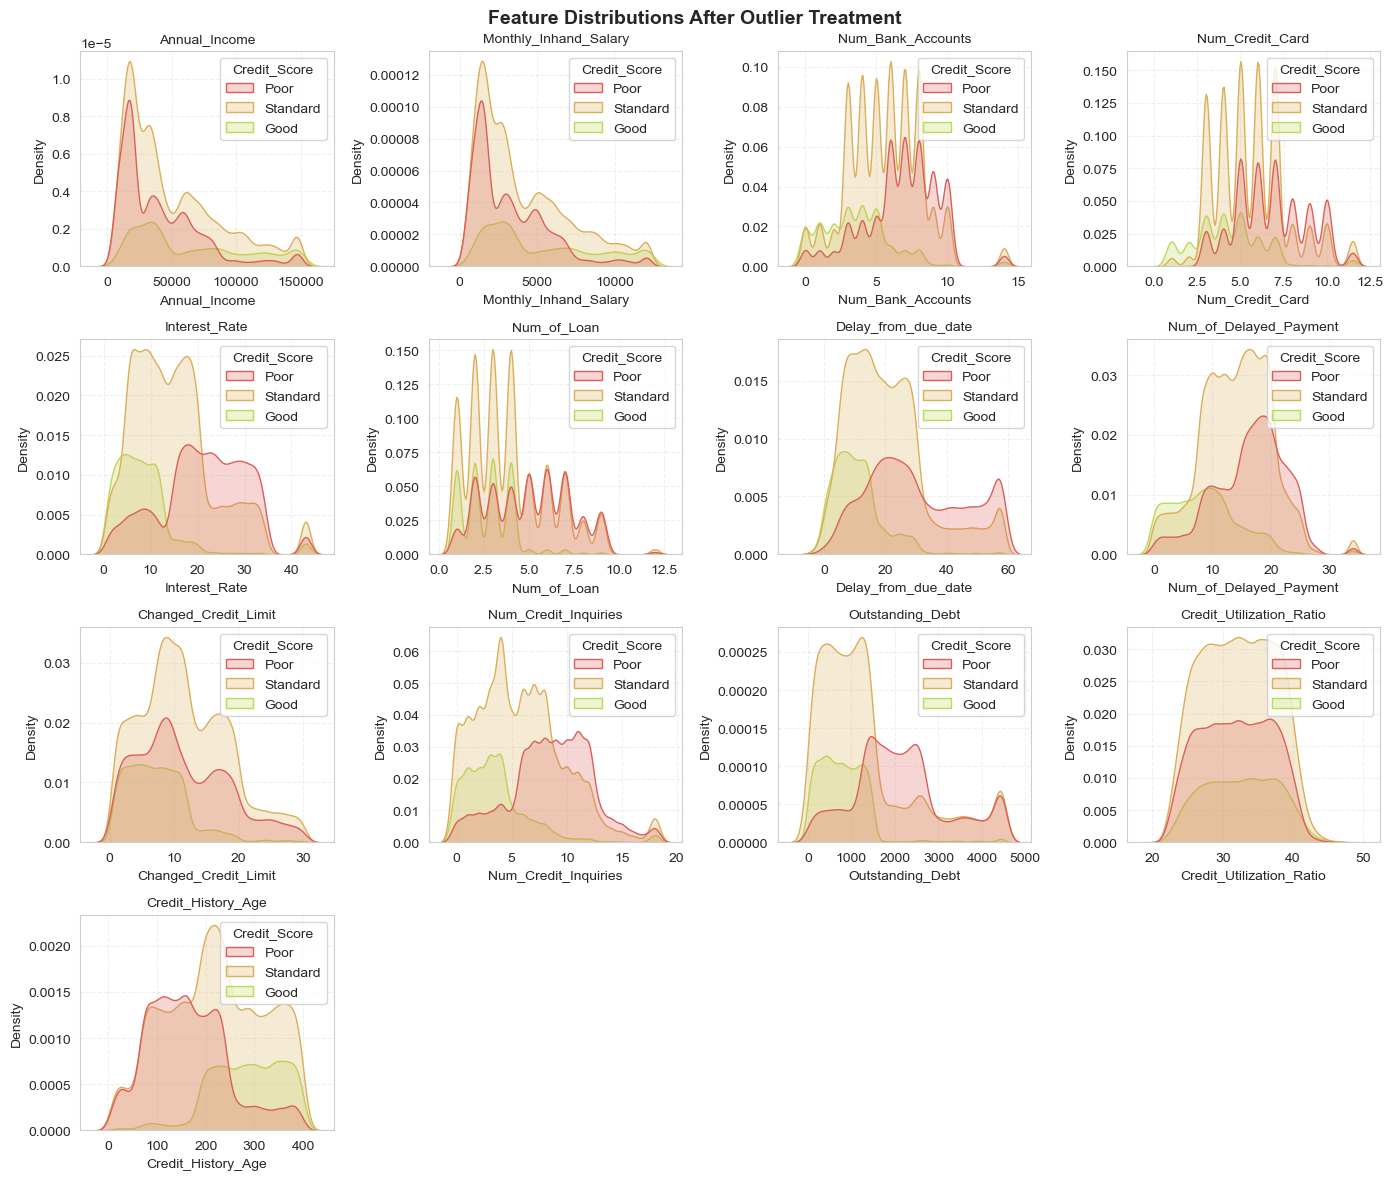
\includegraphics[width=0.9\textwidth]{Feature-out.png}
    \caption{Distribution Comparison: After Preprocessing. The preprocessing pipeline effectively normalized distributions, removed outliers, and improved feature quality.}
    \label{fig:dist_comparison}
\end{figure} 

\section{Methodology \& Models}

We implemented and tuned six distinct models to solve the classification task. A 5-fold Cross-Validation strategy with \texttt{GridSearchCV} was employed for hyperparameter tuning, optimizing for the weighted F1-score.

Figure \ref{fig:corr_matrix} shows the correlation structure among the final 20 selected features, revealing key relationships that inform model performance.

\begin{figure}[h]
    \centering
    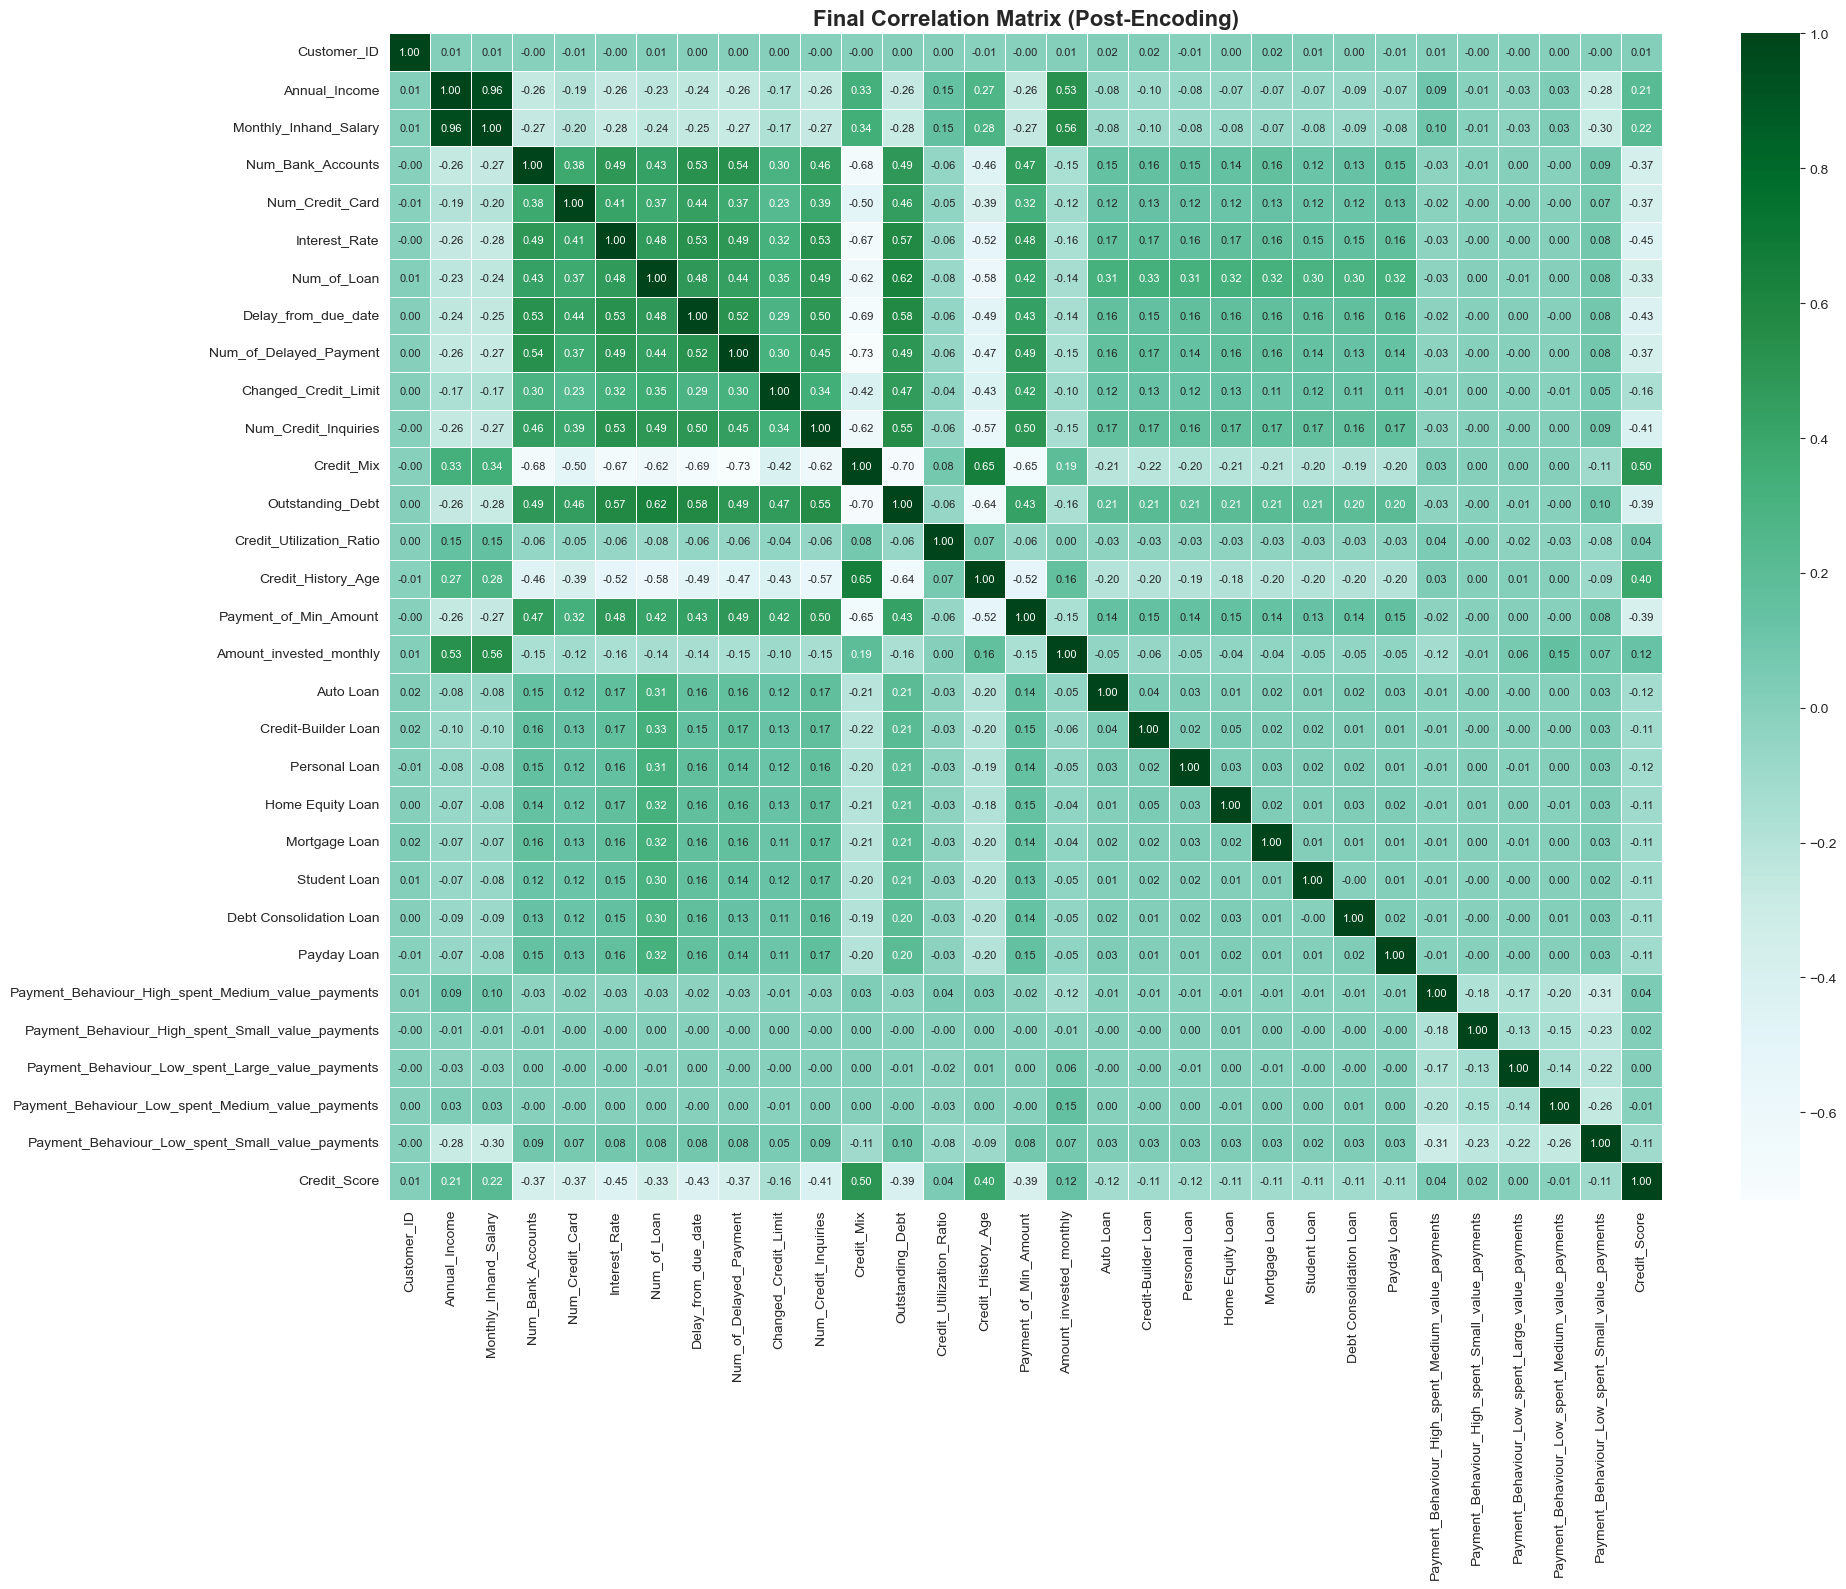
\includegraphics[width=0.85\textwidth]{corr_matrix.png}
    \caption{Correlation Matrix of Top 20 Selected Features. Darker colors indicate stronger correlations, revealing feature relationships that influence model behavior.}
    \label{fig:corr_matrix}
\end{figure}

\subsection{Models Implemented}

\begin{enumerate}
    \item \textbf{Gaussian Naive Bayes:} A probabilistic classifier assuming continuous features follow a Gaussian distribution.
    \begin{itemize}
        \item \textit{Hyperparameters:} \texttt{var\_smoothing} ($10^{-9}$ to $10^{-3}$).
        \item \textit{Scaling:} RobustScaler.
    \end{itemize}

    \item \textbf{Multinomial Naive Bayes:} Suited for discrete counts.
    \begin{itemize}
        \item \textit{Hyperparameters:} \texttt{alpha} (0.1 to 10.0).
        \item \textit{Scaling:} MinMaxScaler (required for non-negative input).
    \end{itemize}

    \item \textbf{Softmax Regression (Logistic Regression):} A linear model generalized for multi-class problems.
    \begin{itemize}
        \item \textit{Hyperparameters:} Regularization strength \texttt{C} (0.001 to 1.0).
        \item \textit{Settings:} L2 penalty, \texttt{class\_weight='balanced'} to handle class imbalance.
        \item \textit{Scaling:} RobustScaler.
    \end{itemize}

    \item \textbf{Decision Tree:} A non-linear model capable of capturing complex decision boundaries.
    \begin{itemize}
        \item \textit{Hyperparameters:} \texttt{max\_depth} (5, 10, 15, None), \texttt{min\_samples\_split}, \texttt{min\_samples\_leaf}, \texttt{criterion} (Gini, Entropy).
        \item \textit{Settings:} \texttt{class\_weight='balanced'}.
    \end{itemize}

    \item \textbf{Random Forest:} An ensemble of decision trees to reduce variance and overfitting.
    \begin{itemize}
        \item \textit{Hyperparameters:} \texttt{n\_estimators} (150, 200), \texttt{max\_depth} (20, 25), \texttt{min\_samples\_split}, \texttt{min\_samples\_leaf}.
        \item \textit{Settings:} \texttt{class\_weight='balanced\_subsample'}.
    \end{itemize}

    \item \textbf{Random Forest (Reduced Features):} A variant of the above model using only the top 15 features (explaining 95\% of cumulative importance) to test efficiency vs. performance trade-offs.
\end{enumerate}

\section{Performance Metrics}

To evaluate the models comprehensively, we utilized the following metrics:
\begin{itemize}
    \item \textbf{Accuracy:} The ratio of correctly predicted observations to total observations.
    \item \textbf{Precision, Recall, F1-Score:} Weighted averages were calculated to account for class imbalance.
    \item \textbf{Confusion Matrix:} To visualize misclassifications between classes.
    \item \textbf{ROC-AUC:} One-vs-Rest approach to measure the ability of the classifier to distinguish between classes.
    \item \textbf{Computational Cost:} Training time measured in seconds.
\end{itemize}

\subsection{Summary of Results}

Table \ref{tab:model_performance} summarizes the performance of all models on the test set.

\begin{table}[H]
    \centering
    \caption{Model Performance Comparison (Test Set)}
    \label{tab:model_performance}
    \begin{tabular}{lcccc}
        \toprule
        \textbf{Model} & \textbf{Accuracy} & \textbf{Precision} & \textbf{Recall} & \textbf{F1 Score} \\
        \midrule
        Gaussian NB & 0.6174 & 0.6826 & 0.6174 & 0.6197 \\
        Multinomial NB & 0.5780 & 0.5714 & 0.5780 & 0.5598 \\
        Softmax Regression & 0.6535 & 0.6917 & 0.6535 & 0.6570 \\
        Decision Tree & 0.7359 & 0.7560 & 0.7359 & 0.7368 \\
        \textbf{Random Forest (20 Feat.)} & \textbf{0.7920} & \textbf{0.8051} & \textbf{0.7920} & \textbf{0.7928} \\
        Random Forest (15 Feat.) & 0.7886 & 0.8026 & 0.7886 & 0.7897 \\
        \bottomrule
    \end{tabular}
\end{table}

\begin{table}[H]
    \centering
    \caption{Training Performance and Computational Cost}
    \label{tab:training_performance}
    \begin{tabular}{lcccc}
        \toprule
        \textbf{Model} & \textbf{Train F1} & \textbf{Test F1} & \textbf{Gap} & \textbf{Time (s)} \\
        \midrule
        Gaussian NB & 0.6174 & 0.6197 & -0.0024 & 0.09 \\
        Multinomial NB & 0.5611 & 0.5598 & 0.0013 & 0.01 \\
        Softmax Regression & 0.6580 & 0.6570 & 0.0010 & 0.43 \\
        Decision Tree & 0.8187 & 0.7368 & 0.0819 & 1.51 \\
        \textbf{Random Forest (20 Feat.)} & \textbf{0.8583} & \textbf{0.7928} & \textbf{0.0655} & \textbf{28.56} \\
        Random Forest (15 Feat.) & 0.8553 & 0.7897 & 0.0657 & 28.13 \\
        \bottomrule
    \end{tabular}
\end{table}

\begin{table}[H]
    \centering
    \caption{Per-Class Performance for Random Forest (20 Features) - Best Model}
    \label{tab:per_class}
    \begin{tabular}{lcccc}
        \toprule
        \textbf{Class} & \textbf{Precision} & \textbf{Recall} & \textbf{F1 Score} & \textbf{Support} \\
        \midrule
        Poor & 0.77 & 0.87 & 0.82 & 5,533 \\
        Standard & 0.87 & 0.73 & 0.80 & 9,309 \\
        Good & 0.66 & 0.84 & 0.74 & 2,877 \\
        \midrule
        \textbf{Weighted Avg.} & \textbf{0.81} & \textbf{0.79} & \textbf{0.79} & \textbf{17,719} \\
        \bottomrule
    \end{tabular}
\end{table}

\begin{table}[H]
    \centering
    \caption{ROC-AUC Scores (One-vs-Rest) for All Models}
    \label{tab:roc_auc}
    \begin{tabular}{lccc}
        \toprule
        \textbf{Model} & \textbf{Poor vs Rest} & \textbf{Standard vs Rest} & \textbf{Good vs Rest} \\
        \midrule
        Gaussian NB & 0.762 & 0.694 & 0.855 \\
        Multinomial NB & 0.752 & 0.676 & 0.845 \\
        Softmax Regression & 0.794 & 0.738 & 0.872 \\
        Decision Tree & 0.896 & 0.819 & 0.910 \\
        \textbf{Random Forest (20 Feat.)} & \textbf{0.933} & \textbf{0.869} & \textbf{0.956} \\
        Random Forest (15 Feat.) & 0.930 & 0.867 & 0.954 \\
        \bottomrule
    \end{tabular}
\end{table}

\begin{figure}[H]
    \centering
    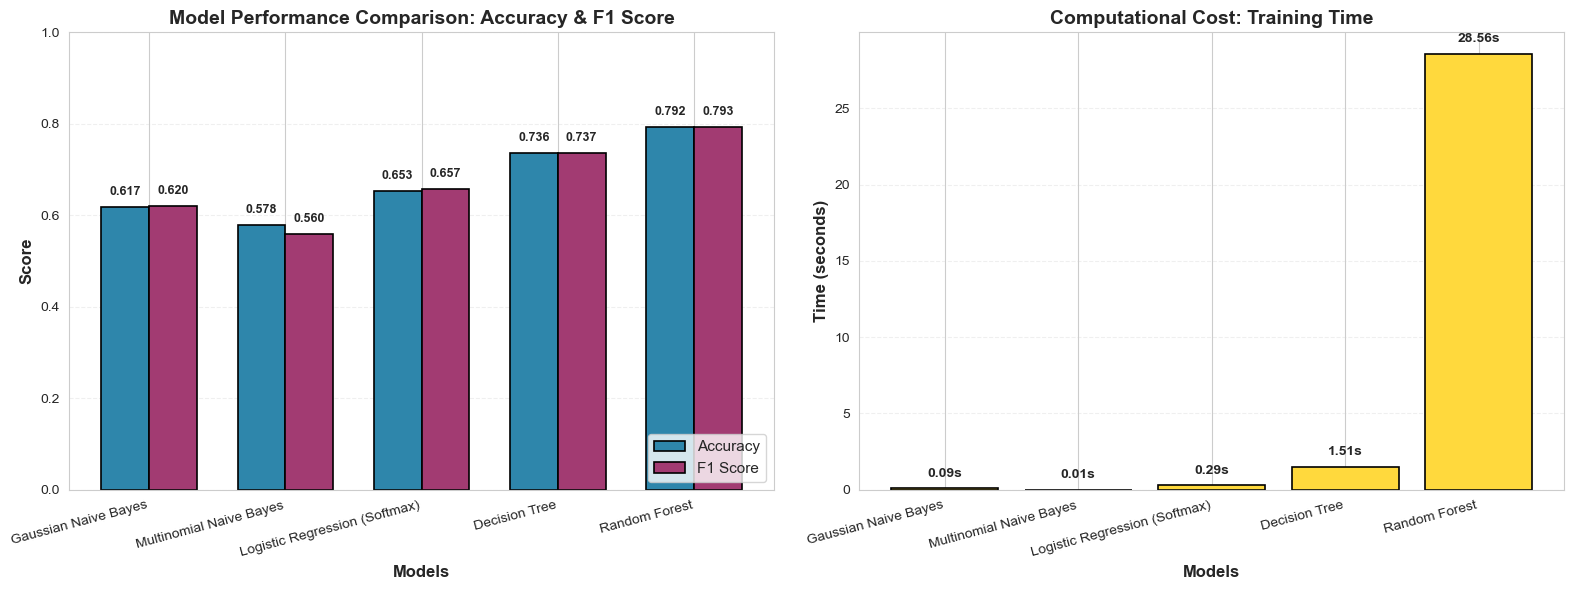
\includegraphics[width=1\textwidth]{Accuracy_F1_TrainingTime.png}
    \caption{Comparison of Accuracy \& F1 Scores and Training Time across all models.}
    \label{fig:model_comp}
\end{figure}

\begin{figure}[H]
    \centering
    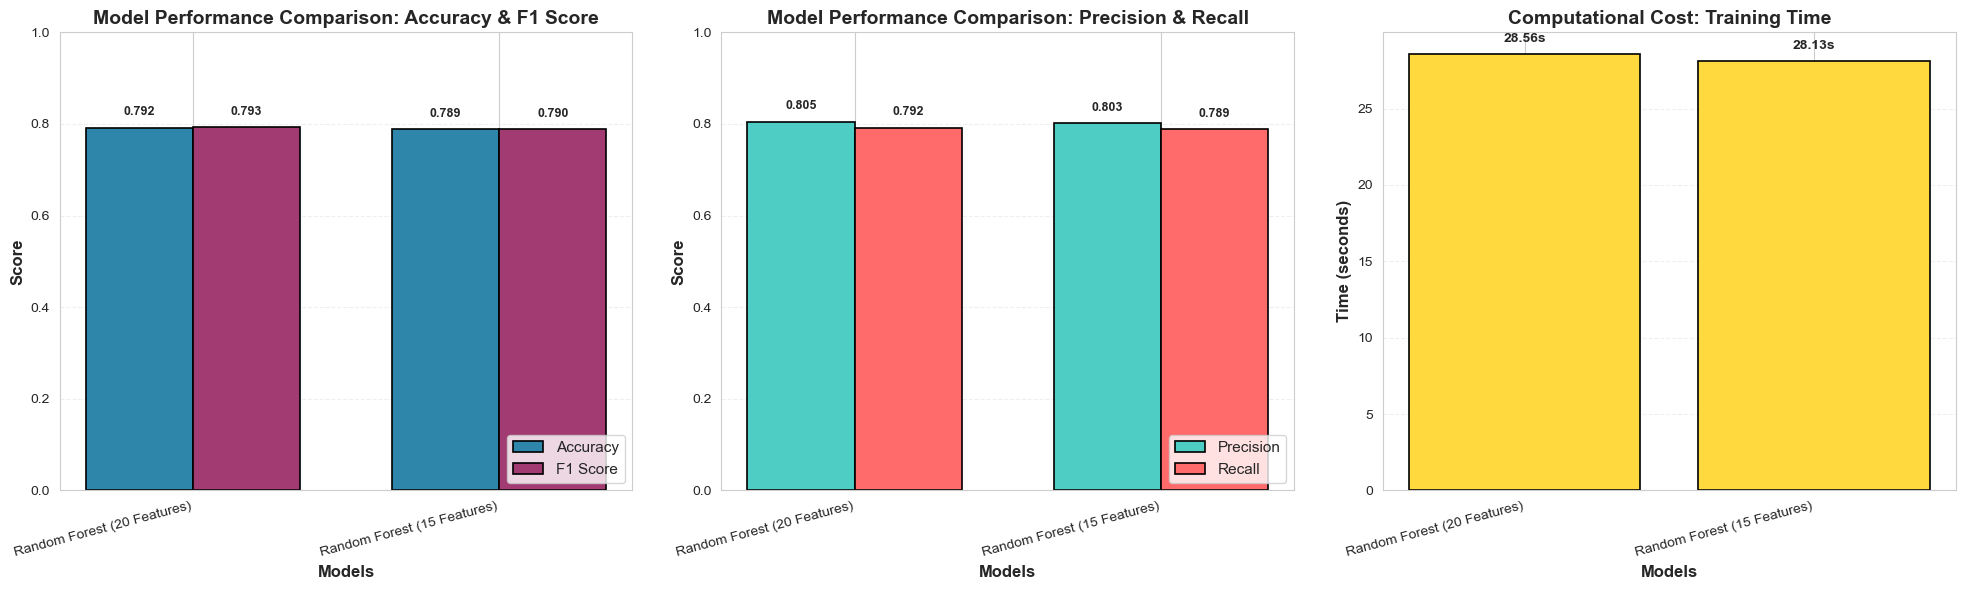
\includegraphics[width=1\textwidth]{rfvsrf.png}
    \caption{Comprehensive comparison of Random Forest variants (20 vs 15 features) across all performance metrics.}
    \label{fig:rf_comparison}
\end{figure}

\begin{figure}[H]
    \centering
    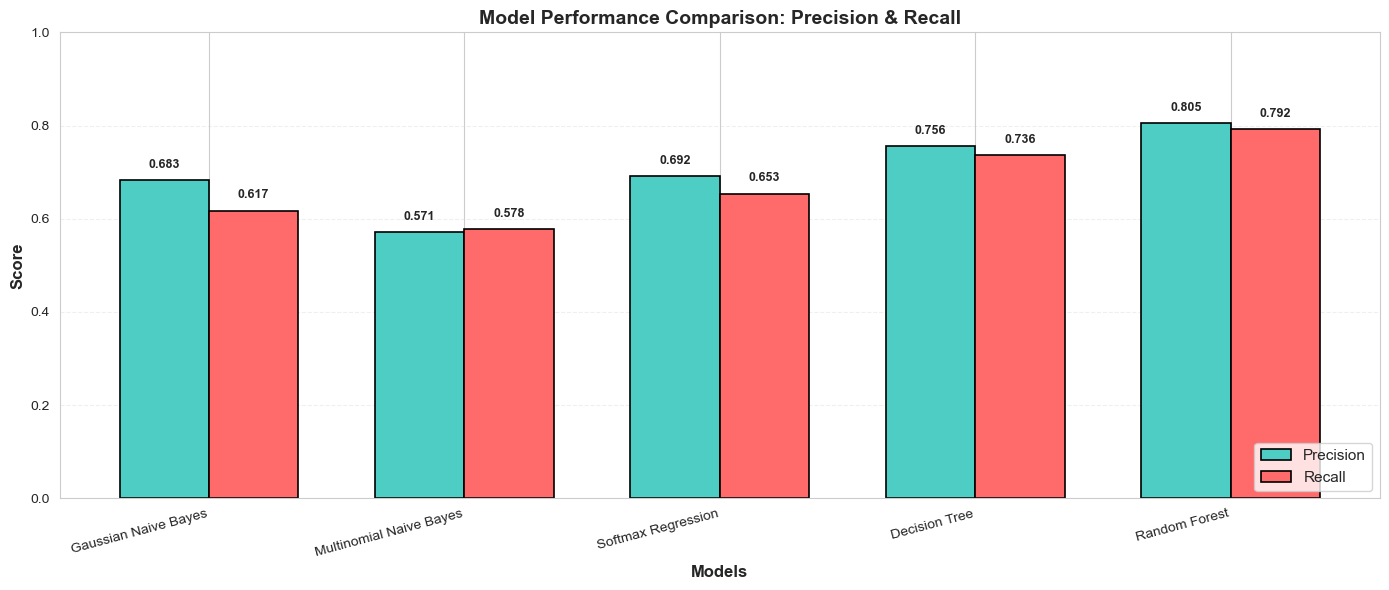
\includegraphics[width=0.9\textwidth]{prec_rec.png}
    \caption{Precision-Recall histograms for all models showing trade-offs between precision and recall.}
    \label{fig:pr_curve}
\end{figure}

\begin{figure}[H]
    \centering
    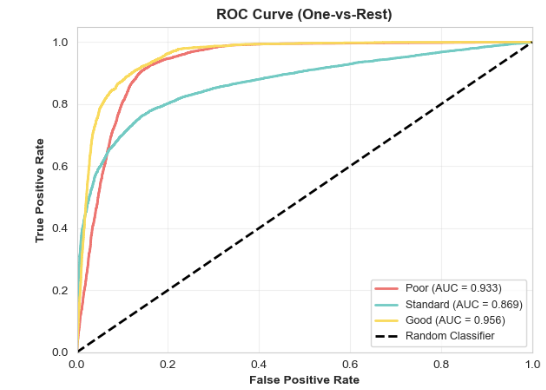
\includegraphics[width=0.6\textwidth]{roc.png}
    \caption{ROC curves (One-vs-Rest) for Random Forest showing discrimination ability for each class.}
    \label{fig:roc_curves}
\end{figure}

\section{Results \& Analysis}

\subsection{Model Performance and Comparative Analysis}

\subsubsection{Performance Hierarchy}
\textbf{Random Forest (20 features)} achieved the best performance with F1=0.7928 and accuracy=0.7920, substantially outperforming all alternatives:
\begin{enumerate}
    \item Random Forest (20 feat.): F1 = 0.7928
    \item Random Forest (15 feat.): F1 = 0.7897 (0.31\% lower)
    \item Decision Tree: F1 = 0.7368 (5.60\% lower)
    \item Softmax Regression: F1 = 0.6570 (13.58\% lower)
    \item Gaussian NB: F1 = 0.6197 (17.31\% lower)
    \item Multinomial NB: F1 = 0.5598 (23.30\% lower)
\end{enumerate}

\subsubsection{Why Random Forest Excels}
Random Forest's superiority stems from four key advantages:

\begin{enumerate}
    \item \textbf{Ensemble learning}: 200 diverse trees reduce variance through democratic voting, improving single Decision Tree performance by 5.6\%.
    \item \textbf{Non-linear pattern recognition}: Recursive partitioning captures complex relationships (such as U-shaped credit utilization curves) that linear models miss.
    \item \textbf{Feature interaction modeling}: Tree paths implicitly model interactions like ``high debt AND low income implies poor credit''.
    \item \textbf{Noise robustness}: Bagging averages out measurement errors across bootstrap samples.
\end{enumerate}

The 15-feature variant achieves F1=0.7897 (only 0.31\% lower), demonstrating that 25\% of features contribute negligible value and can be removed for simpler deployment.

\subsubsection{Impact of Model Assumptions}

\textbf{Naive Bayes} (Gaussian F1=0.6197, Multinomial F1=0.5598) underperformed due to violated assumptions. First, feature independence is violated because credit features exhibit strong correlations, such as Annual Income with Monthly Salary, and Outstanding Debt with EMI payments. This violates the independence assumption $P(X_1,...,X_n|Y)=\prod P(X_i|Y)$. Second, distributional assumptions fail because financial data shows heavy tails and multimodality rather than Gaussian distributions. Multinomial NB assumes discrete counts, which is inappropriate for continuous variables.

\textbf{Softmax Regression} (F1=0.6570) suffers from linear boundary limitations. Credit relationships are non-linear. For example, credit utilization shows U-shaped risk where both 0\% and 100\% are problematic, and feature interactions such as high debt combined with low income cannot be captured without explicit engineering. However, 65.7\% F1 indicates some linear structure exists, justifying its use as a fast baseline.

\textbf{Tree-Based Models} excel due to assumption-free learning. They have no distributional requirements, automatically capture non-linearity through recursive partitioning, implicitly model interactions via tree paths, and seamlessly handle mixed data types.

\subsubsection{Overfitting Analysis}

Table \ref{tab:overfitting} shows train-test F1 gaps quantifying overfitting. We classify models with gaps exceeding 0.10 as overfitting.

\begin{table}[H]
    \centering
    \caption{Overfitting Analysis (Overfitting threshold: gap > 0.10)}
    \label{tab:overfitting}
    \begin{tabular}{lcccc}
        \toprule
        \textbf{Model} & \textbf{Train F1} & \textbf{Test F1} & \textbf{Gap} & \textbf{Status} \\
        \midrule
        Gaussian NB & 0.6174 & 0.6197 & -0.0024 & Underfitting \\
        Multinomial NB & 0.5611 & 0.5598 & 0.0013 & Underfitting \\
        Softmax Regression & 0.6580 & 0.6570 & 0.0010 & Excellent \\
        Decision Tree & 0.8187 & 0.7368 & 0.0819 & Good \\
        Random Forest (20) & 0.8583 & 0.7928 & 0.0655 & Good \\
        Random Forest (15) & 0.8553 & 0.7897 & 0.0657 & Good \\
        \bottomrule
    \end{tabular}
\end{table}

Key findings from overfitting analysis:

\begin{itemize}
    \item \textbf{Decision Tree} shows a gap of 0.0819 (below the 0.10 threshold) by growing deep trees that memorize some training noise, but remains within acceptable bounds.
    
    \item \textbf{Random Forest} reduces the gap to 0.0655 through three mechanisms:
    \begin{enumerate}
        \item Bagging uses 200 bootstrap samples that expose trees to different data, averaging out noise
        \item Feature randomness considers only approximately 4.5 features (square root of 20) per split, decorrelating trees
        \item Balanced class weights adjust for imbalance
    \end{enumerate}
    
    \item \textbf{Naive Bayes} models underfit (negative gaps) because they are too rigid to learn training data effectively.
    
    \item \textbf{Softmax Regression} shows a near-zero gap, but this reflects underfitting rather than excellent generalization.
\end{itemize}

Learning curves (Figure \ref{fig:learning_curves}) show that Random Forest's train-validation gap narrows from 0.10 (with 10\% of data) to 0.07 (with 100\% of data), indicating that more data reduces overfitting. The validation score plateaus at 0.79, suggesting capacity limits. GridSearchCV-optimized hyperparameters (\texttt{max\_depth=25, min\_samples\_split=12, min\_samples\_leaf=4, n\_estimators=200}) provide regularization.

\begin{figure}[H]
    \centering
    \begin{subfigure}[b]{0.45\textwidth}
        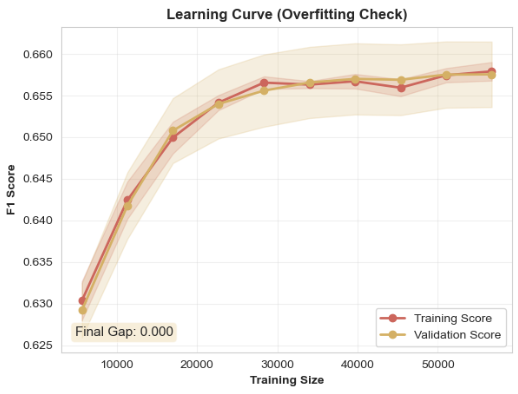
\includegraphics[width=\textwidth]{Dt.png}
        \caption{Decision Tree Learning Curve}
    \end{subfigure}
    \hfill
    \begin{subfigure}[b]{0.45\textwidth}
        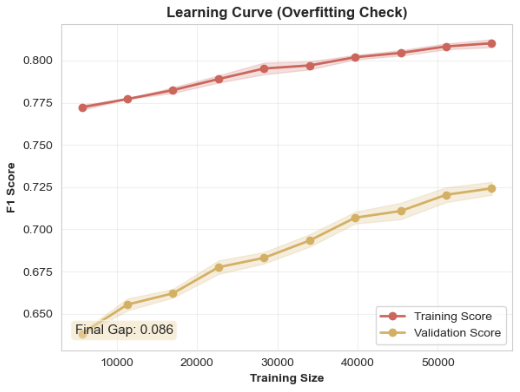
\includegraphics[width=\textwidth]{Rf.png}
        \caption{Random Forest Learning Curve}
    \end{subfigure}
    \caption{Learning curves showing Training vs. Validation scores.}
    \label{fig:learning_curves}
\end{figure}

\subsubsection{Feature Importance}

Figure \ref{fig:feat_imp} shows Random Forest feature importance (mean decrease in Gini impurity).

\begin{figure}[H]
    \centering
    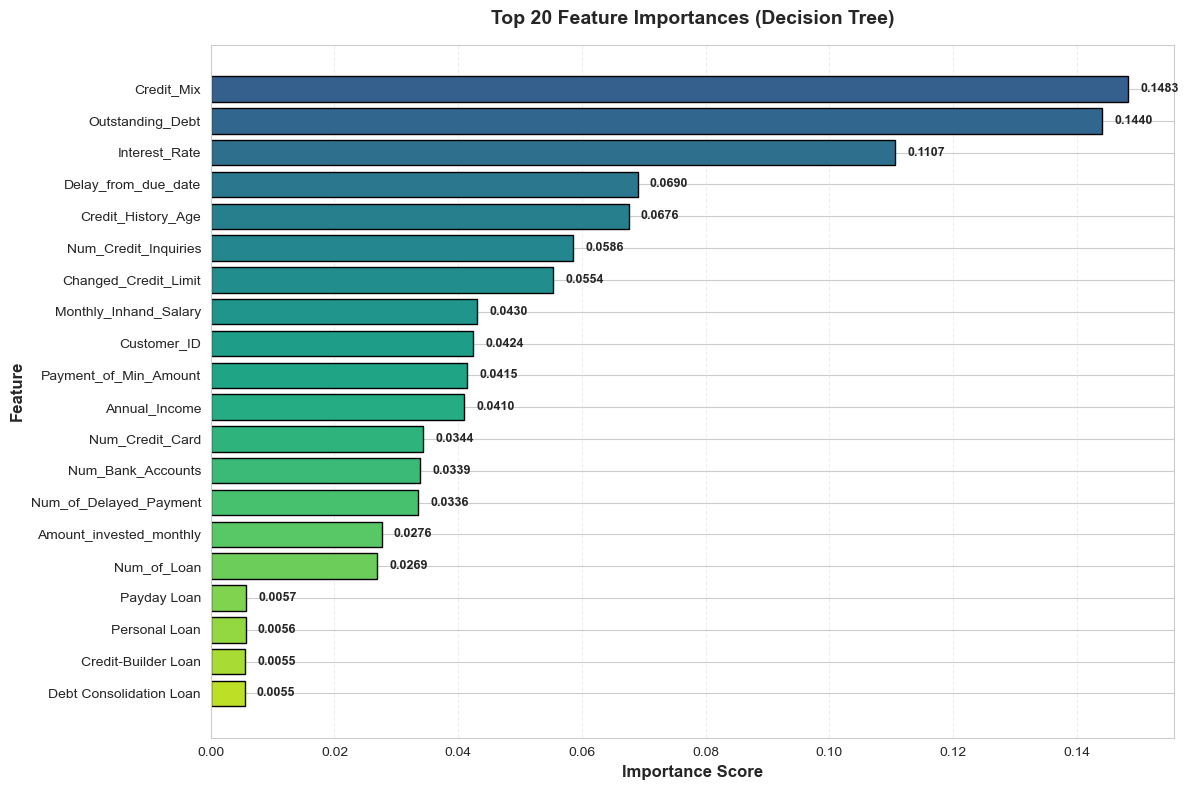
\includegraphics[width=0.85\textwidth]{importance.png}
    \caption{Top 20 Features by Importance.}
    \label{fig:feat_imp}
\end{figure}

The top 3 features account for 40.3\% of total importance:

\begin{itemize}
    \item \textbf{Credit\_Mix (14.83\%)}: Portfolio diversity reflects financial maturity
    \item \textbf{Outstanding\_Debt (14.40\%)}: Debt burden limits repayment capacity
    \item \textbf{Interest\_Rate (11.07\%)}: Encodes historical credit performance
\end{itemize}

Mid-tier features (ranks 4-10, accounting for 27.4\%) capture payment behavior:

\begin{itemize}
    \item Delay\_from\_due\_date: 6.90\%
    \item Credit\_History\_Age: 6.76\%
    \item Num\_Credit\_Inquiries: 5.86\%
    \item Changed\_Credit\_Limit: 5.54\%
    \item Monthly\_Inhand\_Salary: 4.30\% (surprisingly ranks only 8th, suggesting behavior matters more than income)
\end{itemize}

Key insights:

\begin{itemize}
    \item Loan type indicators (ranks 16-20) contribute less than 0.6\% each
    \item The top 15 features explain 95\% of cumulative importance, validating the 15-feature model (F1=0.7897 versus 0.7928)
    \item Age and Occupation were dropped during preprocessing, suggesting that \textit{what you do with credit} matters more than \textit{who you are}, potentially reducing demographic bias
\end{itemize}

\subsubsection{Class-Specific Performance}

Table \ref{tab:per_class} and Figure \ref{fig:conf_matrix} show per-class metrics for Random Forest.

\begin{figure}[H]
    \centering
    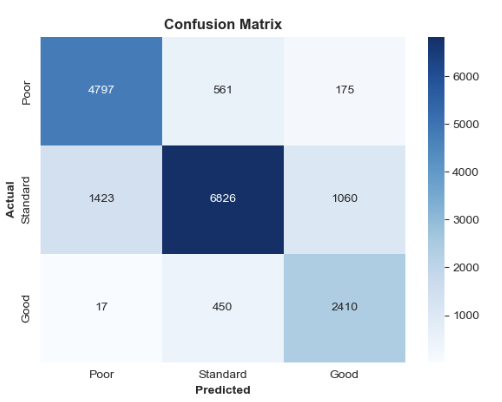
\includegraphics[width=0.5\textwidth]{cf_rf.png}
    \caption{Confusion Matrix for Random Forest.}
    \label{fig:conf_matrix}
\end{figure}

\textbf{Poor Class} (F1=0.82):
\begin{itemize}
    \item Highest F1 score with precision=0.77 and recall=0.87
    \item High recall captures 87\% of risky customers
    \item 23\% false positive rate: 1,423 Standard customers misclassified as Poor, denying credit to eligible applicants
\end{itemize}

\textbf{Standard Class} (F1=0.80):
\begin{itemize}
    \item Highest precision (0.87) but lowest recall (0.73)
    \item Misses 27\% of true Standard customers: 1,423 misclassified as Poor, 1,060 as Good
    \item As the majority class (52.5\% of data), the model favors precision over recall
\end{itemize}

\textbf{Good Class} (F1=0.74):
\begin{itemize}
    \item Lowest precision (0.66) due to minority status (16.2\% of data)
    \item Captures 84\% of good credit customers but produces 34\% false positives
    \item High AUC (0.956) suggests good ranking ability; threshold tuning could improve precision
\end{itemize}

\textbf{Key Error Patterns:}
\begin{enumerate}
    \item 1,423 Standard customers misclassified as Poor $\rightarrow$ denies credit to eligible applicants
    \item 1,060 Standard customers misclassified as Good $\rightarrow$ approves moderate-risk customers at favorable terms
    \item 561 Poor customers misclassified as Standard $\rightarrow$ exposes lenders to default risk
\end{enumerate}

\textbf{ROC-AUC Analysis (Figure \ref{fig:roc_curves}):}
\begin{itemize}
    \item Poor vs Rest: 0.933 (excellent discrimination)
    \item Standard vs Rest: 0.869 (weakest due to overlap with both extremes)
    \item Good vs Rest: 0.956 (best discrimination)
    \item High AUC with low precision for Good class indicates threshold calibration issue rather than ranking problem
\end{itemize}

Figure \ref{fig:pr_curve} shows the precision-recall trade-offs for all models, highlighting that Random Forest achieves superior balance across all operating points.

\subsubsection{Computational Cost}

Training times (Table \ref{tab:training_performance}) vary by a factor of 3,000:

\begin{itemize}
    \item \textbf{Fastest}: Naive Bayes (9-86 milliseconds)
    \item \textbf{Moderate}: Softmax Regression (0.429 seconds) - best speed-accuracy compromise
    \item \textbf{Slowest}: Random Forest (28.56 seconds for 20 features, 28.13 seconds for 15 features)
    \begin{itemize}
        \item Trains 200 trees $\times$ 5 CV folds = 1,000 tree trainings
        \item Acceptable for monthly retraining schedules
    \end{itemize}
\end{itemize}

\textbf{Deployment Recommendations:}

\begin{enumerate}
    \item \textbf{Batch Processing:}
    \begin{itemize}
        \item Use Random Forest (20 features) to maximize accuracy
        \item Training overhead negligible for monthly/quarterly updates
    \end{itemize}
    
    \item \textbf{Real-Time APIs:}
    \begin{itemize}
        \item Option 1: Random Forest (15 features) - 28.13s training, 1-5ms inference
        \item Option 2: Softmax Regression - 0.43s training, F1=0.6570
        \item RF inference supports 500 predictions/second on single CPU core
    \end{itemize}
    
    \item \textbf{High-Frequency Retraining:}
    \begin{itemize}
        \item Use Softmax Regression for sub-second retraining cycles
    \end{itemize}
\end{enumerate}

\textbf{Performance Optimization:}

\begin{itemize}
    \item \textbf{Parallelization}: 16-core CPU reduces RF training to 3-5 seconds
    \item \textbf{GPU Acceleration}: Achieves 10-100$\times$ speedup
    \item \textbf{Inference Time}: RF (0.5-2ms/sample) vs Softmax (0.005ms/sample)
\end{itemize}

Figure \ref{fig:rf_comparison} provides a comprehensive comparison between the 20-feature and 15-feature Random Forest variants, showing minimal performance degradation with 25\% feature reduction.

\section{Conclusion}

This study successfully developed and evaluated a comprehensive machine learning pipeline for multi-class credit score classification. Through rigorous preprocessing and systematic comparison of six algorithms, we transformed a raw dataset of 100,000 customer records into actionable predictive models suitable for deployment in financial institutions.

\subsection{Key Findings}

\textbf{Best Model Performance:}
\begin{itemize}
    \item Random Forest (20 features) achieved F1=0.7928, Accuracy=0.7920
    \item Train-test gap=0.0655 (below 0.10 threshold, indicating good generalization)
    \item ROC-AUC scores: Poor (0.933), Standard (0.869), Good (0.956)
\end{itemize}

\textbf{Feature Importance Insights:}
\begin{itemize}
    \item Top 3 features account for 40.3\% of importance:
    \begin{enumerate}
        \item Credit\_Mix: 14.83\%
        \item Outstanding\_Debt: 14.40\%
        \item Interest\_Rate: 11.07\%
    \end{enumerate}
    \item Top 15 features explain 95\% of importance
    \item 15-feature Random Forest achieves F1=0.7897 (only 0.31\% lower)
\end{itemize}

\textbf{Model Assumptions Impact:}
\begin{itemize}
    \item Naive Bayes underperformed by 17-23\% due to feature independence violations
    \item Softmax Regression achieved 13.58\% lower F1 due to linear boundary limitations
    \item Tree-based models' assumption-free learning proved optimal for heterogeneous credit data
\end{itemize}

\textbf{Overfitting Control:}
\begin{itemize}
    \item Decision Tree gap: 0.0819 (below 0.10 threshold)
    \item Random Forest reduced gap to 0.0655 through:
    \begin{enumerate}
        \item Bagging across 200 bootstrap samples
        \item Feature randomness (approximately 4.5 features per split)
        \item Balanced class weights
    \end{enumerate}
    \item GridSearchCV hyperparameters provide effective regularization
\end{itemize}

\subsection{Practical Implications}

\textbf{Deployment Recommendations by Use Case:}
\begin{enumerate}
    \item \textbf{Batch Processing:}
    \begin{itemize}
        \item Use Random Forest with 20 features to maximize accuracy
        \item Monthly/quarterly retraining schedules easily accommodate 28.56-second training time
    \end{itemize}
    
    \item \textbf{Real-Time Applications:}
    \begin{itemize}
        \item Option 1: Random Forest (15 features) - 1-5ms inference
        \item Option 2: Softmax Regression - 0.43s training for frequent updates
    \end{itemize}
    
    \item \textbf{Explainability Requirements:}
    \begin{itemize}
        \item Focus on top 5 features (account for over 50\% of decisions)
        \item Satisfies regulatory transparency requirements
    \end{itemize}
\end{enumerate}

\textbf{Class-Specific Improvement Strategies:}
\begin{itemize}
    \item \textbf{Poor Class (F1=0.82):}
    \begin{itemize}
        \item Reduce 23\% false positive rate
        \item Avoid denying credit to 1,423 misclassified Standard customers
        \item Implement secondary review process for borderline cases
    \end{itemize}
    
    \item \textbf{Standard Class (F1=0.80):}
    \begin{itemize}
        \item Improve 73\% recall through enhanced features
        \item Implement secondary manual reviews for edge cases
        \item Target the 2,483 misclassified customers
    \end{itemize}
    
    \item \textbf{Good Class (F1=0.74):}
    \begin{itemize}
        \item Improve 66\% precision using cost-sensitive learning
        \item Apply threshold tuning (high AUC=0.956 indicates good ranking)
        \item Consider collecting more data for minority class (16.2\% of dataset)
    \end{itemize}
\end{itemize}

\subsection{Limitations}

\textbf{Data Limitations:}
\begin{itemize}
    \item Missing key contextual features: employment history, education level
    \item Lacks temporal trends: cross-sectional data ignores credit behavior evolution
    \item No macroeconomic variables: unemployment rate, inflation, interest rate environment
    \item Geographic information absent: models may not generalize across regions
\end{itemize}

\textbf{Modeling Assumptions:}
\begin{itemize}
    \item Assumes Kaggle labels accurately reflect true credit risk
    \item IID assumption violated: correlated economic shocks affect multiple customers simultaneously
    \item Static model: does not account for concept drift or changing credit standards
\end{itemize}

\subsection{Future Work}

\textbf{Advanced Algorithms:}
\begin{itemize}
    \item Evaluate gradient boosting methods (XGBoost, LightGBM, CatBoost)
    \item Expected 2-5\% F1 improvement through sequential error correction
    \item Temporal models (LSTMs) to capture credit trajectory trends over time
\end{itemize}

\textbf{Enhanced Feature Engineering:}
\begin{itemize}
    \item Polynomial interactions: $Outstanding\_Debt \times Interest\_Rate$
    \item Derived ratios: debt-to-income, credit utilization trends
    \item Temporal features: payment consistency, credit mix evolution
\end{itemize}

\textbf{Class Imbalance Techniques:}
\begin{itemize}
    \item Note: SMOTE and SMOTE+Tomek were tested but yielded worse performance than balanced class weights
    \item Explore cost-sensitive learning with asymmetric misclassification penalties
    \item Threshold optimization per class using precision-recall curves
\end{itemize}

\textbf{Model Validation:}
\begin{itemize}
    \item Fairness auditing to ensure equitable lending practices
    \item Adversarial testing for robustness
    \item External validation on different credit score datasets
\end{itemize}

\subsection{Concluding Remarks}

This study demonstrates that machine learning can significantly enhance credit scoring accuracy while maintaining interpretability:

\begin{itemize}
    \item \textbf{Production-Ready Performance:} Random Forest achieved 79.2\% accuracy (F1=0.7928) with good generalization (train-test gap=0.0655, below the 0.10 overfitting threshold).
    
    \item \textbf{Behavior Over Demographics:} Behavioral features (Credit\_Mix, Outstanding\_Debt, Payment Delays) vastly outweigh demographics (Age and Occupation were dropped), suggesting a paradigm shift toward behavior-centric scoring that potentially reduces historical biases.
    
    \item \textbf{Interpretable ML:} Feature importance analysis and ROC-AUC curves provide the transparency required in regulated financial contexts, enabling explainable credit decisions.
    
    \item \textbf{Practical Deployment:} The model supports multiple deployment scenarios from batch processing to real-time APIs, with inference times of 1-5 milliseconds per prediction.
    
    \item \textbf{Future Potential:} Integration of temporal modeling, advanced ensemble methods, and fairness-aware learning could push performance toward the 85-90\% F1 frontier.
\end{itemize}

The convergence of rigorous preprocessing, assumption-free learning, and comprehensive evaluation positions ensemble methods as the foundation for next-generation credit risk assessment systems.

\end{document}
